% !TeX spellcheck = <none>
\documentclass[10pt,twocolumn,letterpaper,english]{article}

\usepackage{cvpr}
\usepackage{times}
\usepackage{epsfig}
\usepackage{graphicx}
\usepackage{amsmath}
\usepackage{amssymb}
\usepackage{listings}
\usepackage{xcolor}
\usepackage{hyperref}
\usepackage{float}

\definecolor{keywords}{RGB}{0,0,255}
\definecolor{comments}{RGB}{0,128,0}
\definecolor{strings}{RGB}{255,0,0}
\definecolor{background}{RGB}{245,245,245}

\lstdefinestyle{cppstyle}{
	language=C++,
	backgroundcolor=\color{background},
	basicstyle=\ttfamily\small,
	keywordstyle=\color{keywords}\bfseries,
	commentstyle=\color{comments}\itshape,
	stringstyle=\color{strings},
	numbers=left,
	numberstyle=\tiny\color{gray},
	stepnumber=1,
	numbersep=5pt,
	tabsize=4,
	breaklines=true,
	showspaces=false,
	showstringspaces=false,
	escapeinside={(*@}{@*)}
}

\lstdefinestyle{compactcode}{
	basicstyle=\small\ttfamily,
	breaklines=true,
	showstringspaces=false,
	breakatwhitespace=true,
	breakindent=0pt,
	escapeinside={(*@}{@*)},
	frame=single,
	aboveskip=2pt,
	belowskip=2pt
}

\usepackage{url}

% Include other packages here, before hyperref.

% If you comment hyperref and then uncomment it, you should delete
% egpaper.aux before re-running latex.  (Or just hit 'q' on the first latex
% run, let it finish, and you should be clear).


\cvprfinalcopy % *** Uncomment this line for the final submission

\def\cvprPaperID{****} % *** Enter the CVPR Paper ID here
\def\httilde{\mbox{\tt\raisebox{-.5ex}{\symbol{126}}}}

% Pages are numbered in submission mode, and unnumbered in camera-ready
\ifcvprfinal\pagestyle{empty}\fi
\begin{document}

%%%%%%%%% TITLE
\title{PC-2023/24 Alpha-Compositor}

\author{Christian Mancini\\
E-mail address\\
{\tt\small christian.mancini1@edu.unifi.it}
% For a paper whose authors are all at the same institution,
% omit the following lines up until the closing ``}''.
% Additional authors and addresses can be added with ``\and'',
% just like the second author.
% To save space, use either the email address or home page, not both
}

\maketitle
\thispagestyle{empty}

%%%%%%%%% ABSTRACT
\begin{abstract}
In this report, we present the implementation of a parallel version of alpha compositing using C++ and OpenMP \cite{openmp}, achieving a speedup of nearly five times. We tested various combinations, including HD to Full HD, Full HD to 2K, and 2K to 4K, while varying the number of threads and images processed.
\end{abstract}

%%%%%%%%% BODY TEXT
\noindent\large\textbf{Future Distribution Permission}\\
\indent The author(s) of this report give permission for this document to be distributed to Unifi-affiliated students taking future courses.

\section{Introduction}

Alpha compositing or alpha blending is the process of combining one image with a background to create the appearance of partial or full transparency. In a 2D image a color combination is stored for each picture element (pixel), often a combination of red, green and blue (RGB). When alpha compositing is in use, each pixel has an additional numeric value stored in its alpha channel (RGBA), with a value ranging from 0 to 1. A value of 0 means that the pixel is fully transparent and the color in the pixel beneath will show through. A value of 1 means that the pixel is fully opaque. 
With this definition in mind we can produce the effect of drawing the
source pixels on top of the destination pixels (foreground over a background) using the following formula: 
\begin{equation}\label{eq:composting}
	[RGBA]_d = [RGBA]_s + [RGBA]_d(1-A_s)
\end{equation}
For our scope the foreground must be completely opaque. Changing the weights leads to different results. 

%-------------------------------------------------------------------------
\subsection{Compositing Algorithm}

The compositing algorithm is straightforward, we just need to apply the \ref{eq:composting} on every channel of the background image, as shown in listing \ref{compose}.
\begin{lstlisting}[style=cppstyle, language=C, caption={Snippet of compose funcion},label={compose}]

bool OpenMP_compose(const Image &foreground, Image &background) {
	if (foreground.height > background.height | foreground.width > background.width) {
		return false;
	}
	#pragma omp parallel for collapse(2) shared(foreground)
	for (int y = 0; y < foreground.height; ++y) {
		for (int x = 0; x < foreground.width; ++x) {
			
			int backgroundIndex = (y * background.width + x) * STBI_rgb_alpha;
			int foregroundIndex = (y * foreground.width + x) * STBI_rgb_alpha;
			
			float alpha = static_cast<float>(foreground.rgb_image[foregroundIndex + 3]) / 255.0f;
			float beta = 1.0f - alpha;
			#pragma omp simd
			for (int color = 0; color < 3; ++color) {
				background.rgb_image[backgroundIndex + color] =
				static_cast<float>(background.rgb_image[backgroundIndex + color]) * beta
				+ static_cast<float>(foreground.rgb_image[foregroundIndex + color]) * alpha;
				
			}
		}
	}
	return true;
}

\end{lstlisting}

%-------------------------------------------------------------------------

\section{Results}

Tables  \ref{tab:fullhd}, \ref{tab:2k}, \ref{tab:4k} shows compositing results and speed up, groupped by the background resolution.

\begin{table}[h]
	\centering
	\caption{FullHD result}
	\begin{tabular}{|c|c|c|c|}
		\hline
		\textbf{Threads} & \textbf{Composing Time} & \textbf{Background} & \textbf{Speedup} \\
		\hline
		1   & 0.3958 & FullHD & 1.0 \\
		25  & 0.1198 & FullHD & 3.3038 \\
		50  & 0.1126 & FullHD & 3.5151 \\
		100 & 0.1195 & FullHD & 3.3121 \\
		200 & 0.1409 & FullHD & 2.8091 \\
		400 & 0.1965 & FullHD & 2.0142 \\
		\hline
	\end{tabular}
	\label{tab:fullhd}
\end{table}

\begin{table}[h]
	\centering
	\caption{2K result}
	\begin{tabular}{|c|c|c|c|}
		\hline
		\textbf{Threads} & \textbf{Composing Time} & \textbf{Background} & \textbf{Speedup} \\
		\hline
		1   & 1.0272 & 2K     & 1.0 \\
		25  & 0.2661 & 2K     & 3.8602 \\
		50  & 0.2511 & 2K     & 4.0908 \\
		100 & 0.2250 & 2K     & 4.5653 \\
		200 & 0.2535 & 2K     & 4.0521 \\
		400 & 0.2866 & 2K     & 3.5841 \\
		\hline
	\end{tabular}
	\label{tab:2k}
\end{table}

\begin{table}[h]
	\centering
	\caption{4K result}
	\begin{tabular}{|c|c|c|c|}
		\hline
		\textbf{Threads} & \textbf{Composing Time} & \textbf{Background} & \textbf{Speedup} \\
		\hline
		1   & 2.0763 & 4K     & 1.0 \\
		25  & 0.4922 & 4K     & 4.2184 \\
		50  & 0.4668 & 4K     & 4.4479 \\
		100 & 0.4276 & 4K     & 4.8557 \\
		200 & 0.4343 & 4K     & 4.7808 \\
		400 & 0.4688 & 4K     & 4.4290 \\
		\hline
	\end{tabular}
	\label{tab:4k}
\end{table}

In Figure \ref{fig:compositing} we show the compositing result of a Background image in 4K and a Foreground in 2K.

\begin{figure}[H]
	\caption{Compositing result example, 2K over 4K}
	\centering
	\label{fig:compositing}
	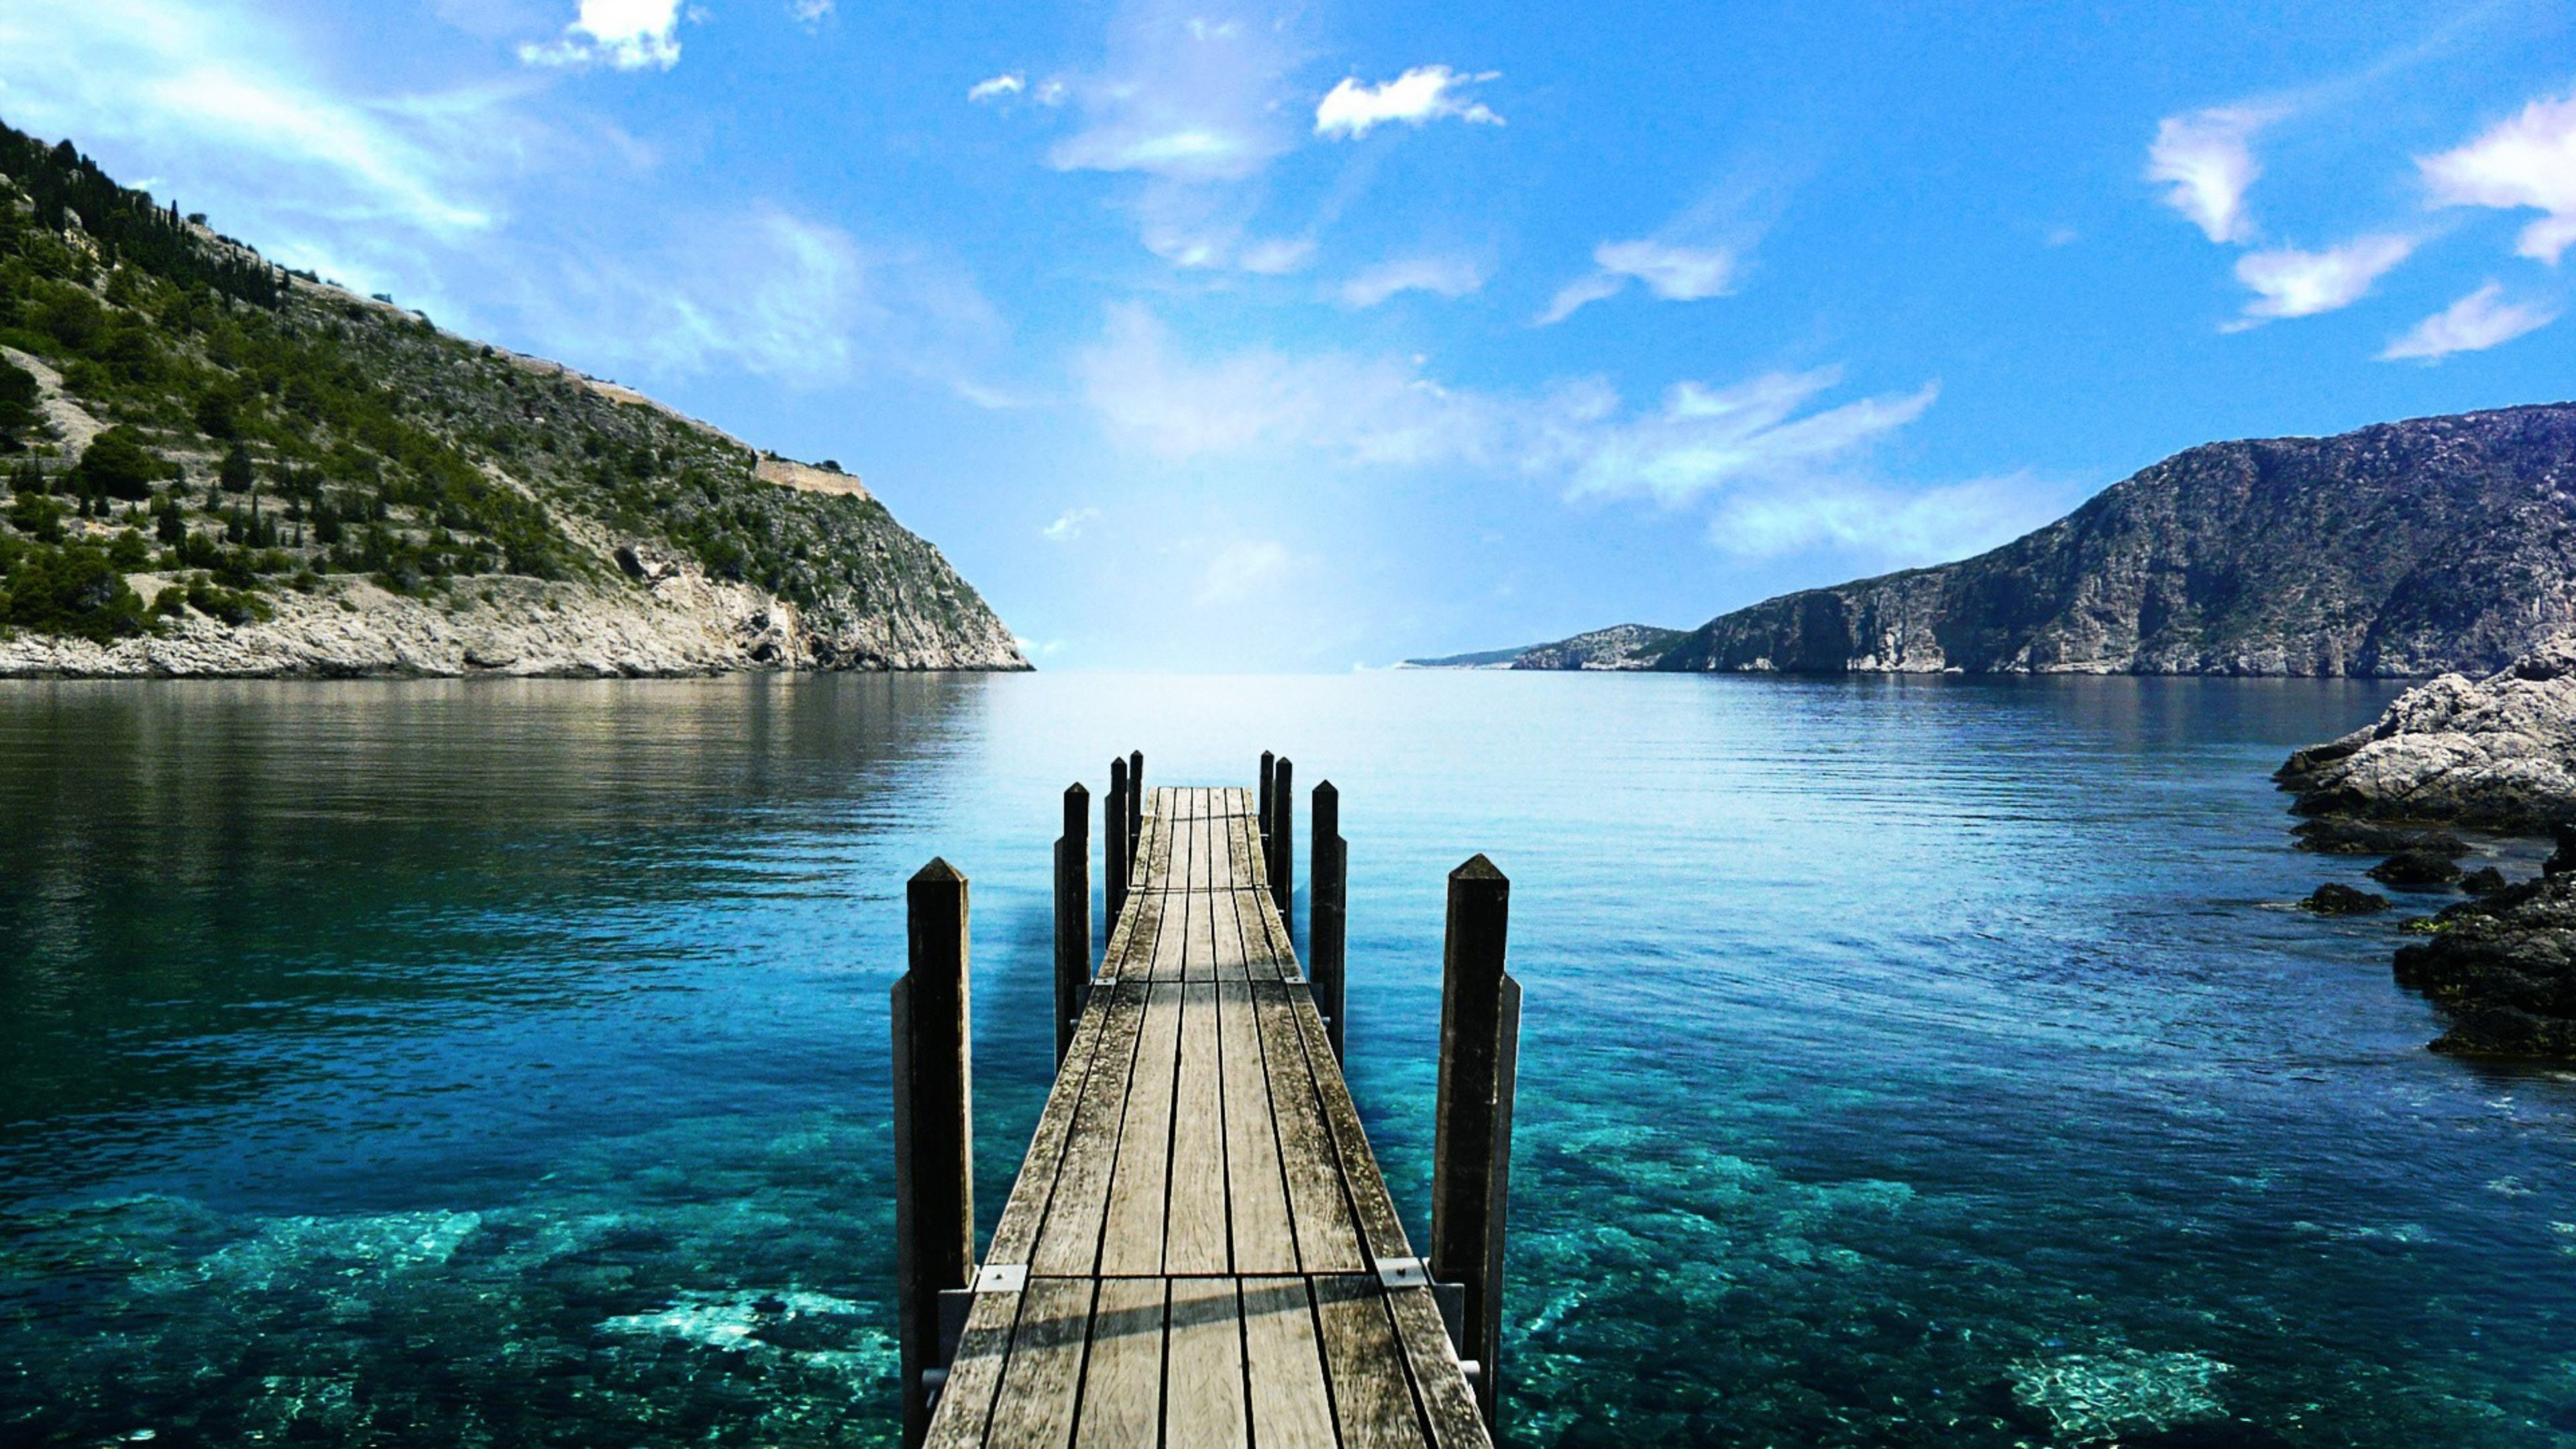
\includegraphics[width=0.5\textwidth]{../Output/4K.png}
\end{figure}

In Figuers \ref{fig:fullhd}, \ref{fig:2K}  and \ref{fig:4K} we show the bar plots of the resoults

\begin{figure}[H]
	\caption{SpeedUp on FullHD Backgroung}
	\centering
	\label{fig:fullhd}
	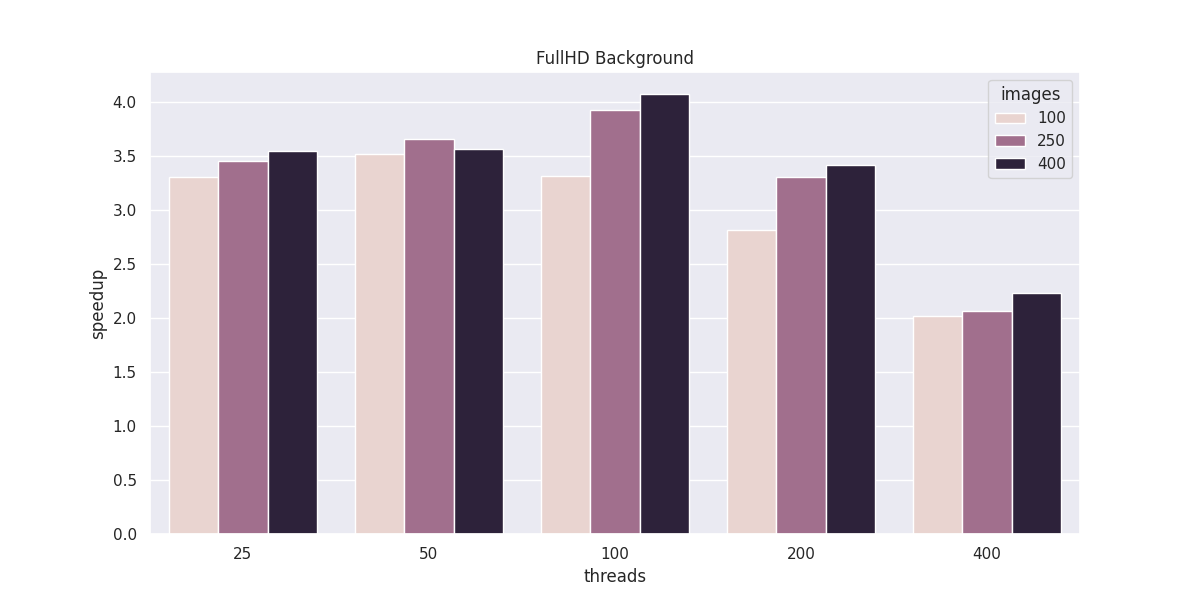
\includegraphics[width=0.6\textwidth]{../plots/fullhd.png}
\end{figure}

\begin{figure}[H]
	\caption{SpeedUp on 2K Backgroung}
	\centering
	\label{fig:2K}
	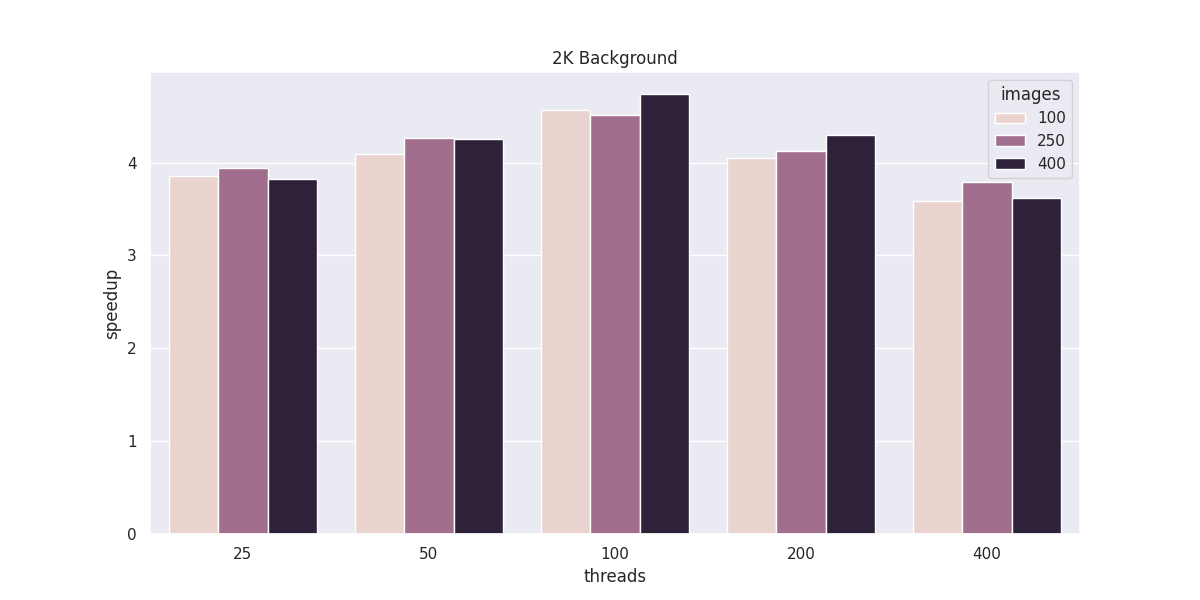
\includegraphics[width=0.6\textwidth]{../plots/2k.png}
\end{figure}

\begin{figure}[H]
	\caption{SpeedUp on 4K Backgroung}
	\centering
	\label{fig:4K}
	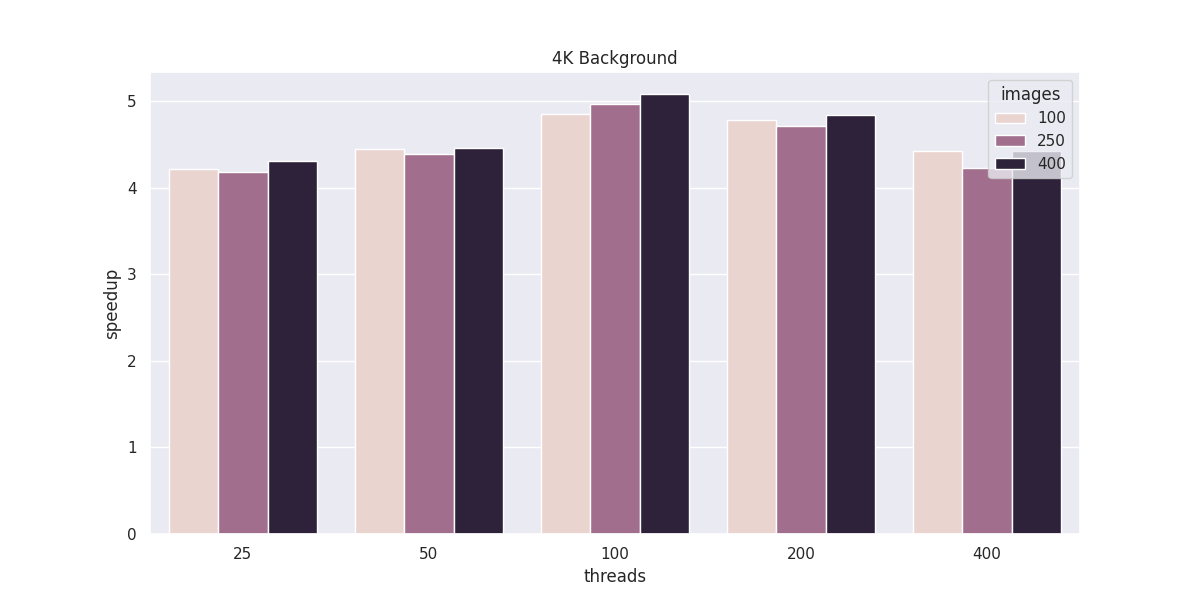
\includegraphics[width=0.6\textwidth]{../plots/4k.png}
\end{figure}



{\small
\bibliographystyle{ieee}
\bibliography{egbib}
}


\end{document}
